%straight line split into angles

\documentclass[tikz,border=10pt]{standalone}
\usepackage{tikz}
\usetikzlibrary{angles,quotes,calc} % Add this for angle labels

\begin{document}

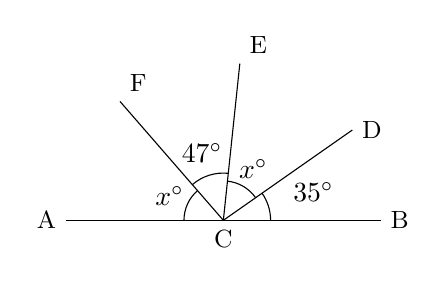
\begin{tikzpicture}[scale=1]
    % Define the points of the cube
    \coordinate (A) at (0,0);
    \coordinate (B) at (4,0);
    \coordinate (C) at (2,0);
    \coordinate (D) at ($(C)+(35:2cm)$);
    \coordinate (E) at ($(C)+(84:2cm)$); 
    \coordinate (F) at ($(C)+(131:2cm)$); 

    % Draw the visible edges of the cube
    \draw (A) -- (B);
    \draw (C) -- (D);
    \draw (C) -- (E);
    \draw (C) -- (F);

    % Draw the angle between lines (C)--(E) and (C)--(F)
    \pic [draw, "$35^{\circ}$", angle eccentricity=2, angle radius=0.6cm] {angle = B--C--D};
    \pic [draw, "$x^{\circ}$", angle eccentricity=1.5] {angle = D--C--E};
    \pic [draw, "$47^{\circ}$", angle eccentricity=1.5, angle radius=0.6cm] {angle = E--C--F};
    \pic [draw, "$x^{\circ}$", angle eccentricity=1.5] {angle = F--C--A};

    % Place the labels with smaller font size
    \node at (A) [left,font=\small] {A};
    \node at (B) [right,font=\small] {B};
    \node at (C) [below,font=\small] {C};
    \node at (D) [right,font=\small] {D};
    \node at (E) [above right,font=\small] {E};
    \node at (F) [above right,font=\small] {F};
    
\end{tikzpicture}

\end{document}